\themaN
\graphicspath{{../../S14_Comparaison_et_egalite_de_fractions/Images/}}

\chapter{Comparaison et\\égalité de fractions}
\label{S14}


%%%%%%%%%%%%%%%%%%%%%%%%%%%%%%%%%%%%%%%
%%%%%%%%%%%%%%%%%%%%%%%%%%%%%%%%%%%%%%%
\begin{prerequis}
   \begin{itemize}
      \item[\com] Effectuer des calculs et des comparaisons de pour traiter des problèmes (fractions).
   \end{itemize}
\end{prerequis}

\vfill

\begin{debat}[Débat : les fractions, ces nombres rompus !] 
   Tout nombre peut s'écrire de différentes façons : ils ont des habillages différents mais ont la même valeur. La façon dont on les écrit permet de pouvoir les comparer. Par exemple, la {\bf fraction} $\dfrac68$ possède (entre autres) les représentations suivantes :
   \begin{center}
      {\psset{unit=0.8}
      \begin{pspicture}(-4,-4)(4,4)  
         \textcolor{B1}{\large
         \multido{\n=5+60,\i=55+60}{6}{\psline(3;\n)(0,0)(3;\i)}
         \multido{\n=30+60,\i=-60+60,\r=120+60}{6}{\psarc(2.719;\n){1.268}{\i}{\r}}
         \pscircle[fillstyle=solid,fillcolor=yellow](0,0){1.3}
         \rput(0,0){\bf $\dfrac68$}
         \rput(2.7;30){75\,\%}
         \rput(2.7;-30){0,75}
         \rput(2.7;150){$\dfrac34$}
         \rput(2.7;-150){$\dfrac{75}{100}$}
         \rput(2.7;90){\pswedge[fillstyle=solid,fillcolor=B3](0,0){0.8}{0}{-90}
                              \pscircle(0,0){0.8}
                              \multido{\n=0+45}{8}{\psline(0,0)(0.8;\n)}}
          \rput(2.7;-90){\psline(-1,0)(1,0)  
          \rput(-1,-0.4){\footnotesize 0}
          \rput(1,-0.4){\footnotesize 1}
          \psline[linecolor=B1,linewidth=1mm](-1,0)(0.5,0) \multido{\r=-1+0.25}{9}{\rput(\r,0){|}}}}
      \end{pspicture}}
   \end{center}
   \bigskip
   \begin{cadre}[B2][F4]
      \begin{center}
         Vidéo : \href{https://www.youtube.com/watch?v=eawBr43xWf8}{\bf Les fractions}, site Internet {\it Le blob}, épisode de la série {\it Petits contes mathématiques}.
      \end{center}
   \end{cadre}
\end{debat}

\vfill

\textcolor{PartieGeometrie}{\sffamily\bfseries Cahier de compétences} : chapitre 2, exercices 1 à 29 ; 43 à 45.


%%%%%%%%%%%%%%%%%%%%%%%%%%%%%%%%%%%%
%%%%%%%%%%%%%%%%%%%%%%%%%%%%%%%%%%%%%
\activites

\begin{activite}[Des briques et des fractions]
   {\bf Objectifs :} utiliser des fractions pour exprimer une proportion ; produire des fractions égales, ranger des fractions. \\
   \begin{QCM}
      \partie[les légo®] \medskip
         \begin{minipage}{10cm}
            On choisit la brique de Lego® classique $u$ ci-contre que l'on prend comme unité et les onze briques $a$ à $k$. On considère que le volume d'une brique est proportionnel au nombre de \og boutons \fg{} présents sur le dessus.
         \end{minipage}
         \hspace{1cm}
         \begin{minipage}{5cm}
            $u$ : 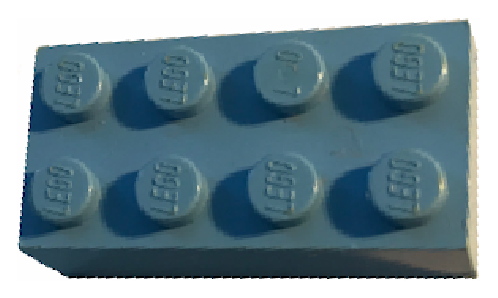
\includegraphics[width=3.15cm]{lego_4_2a}
         \end{minipage} \\ [10mm]
            $a$ : 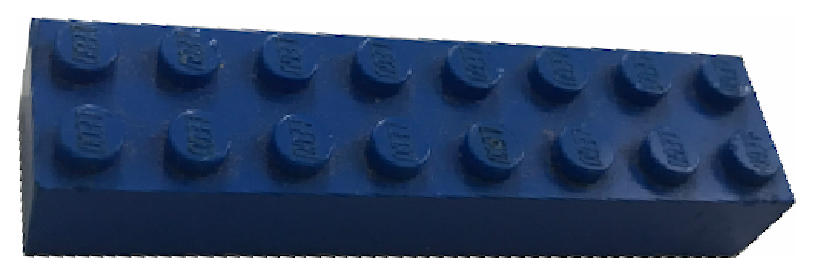
\includegraphics[width=5.22cm]{lego_8_2a} \qquad 
            $b$ : 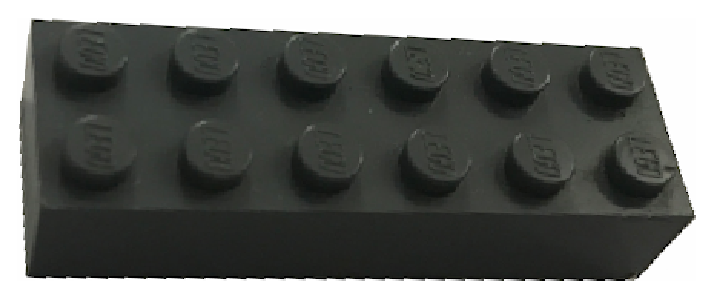
\includegraphics[width=3.6cm]{lego_6_2a} \qquad
            $c$ : 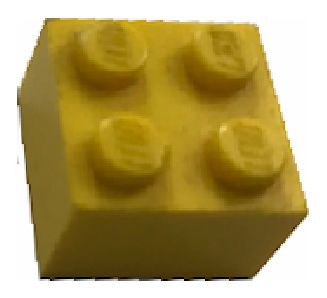
\includegraphics[width=1.35cm]{lego_2_2a} \qquad
            $d$ : 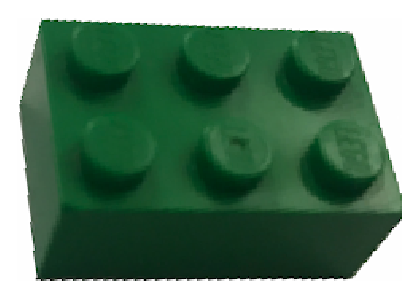
\includegraphics[width=1.8cm]{lego_3_2a} \\ [5mm]
            $e$ : 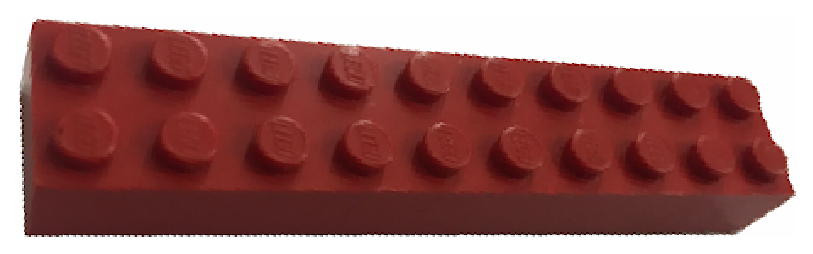
\includegraphics[width=6.3cm]{lego_10_2a} \qquad
            $f$ : 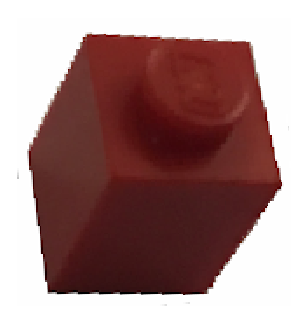
\includegraphics[width=0.9cm]{lego_1_1a} \qquad
            $g$ : 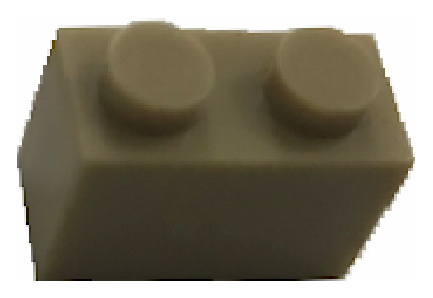
\includegraphics[width=1.35cm]{lego_2_1a} \qquad
            $h$ : 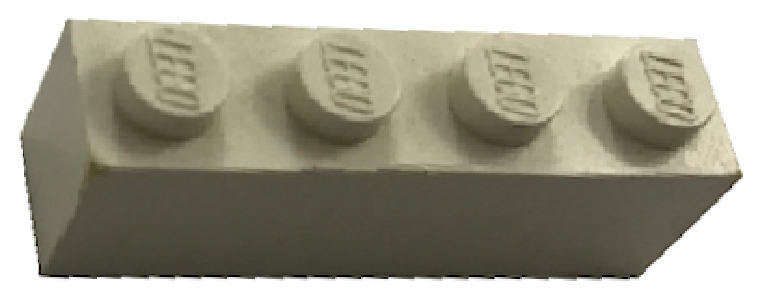
\includegraphics[width=2.7cm]{lego_4_1a} \\ [5mm]
            $i$ : 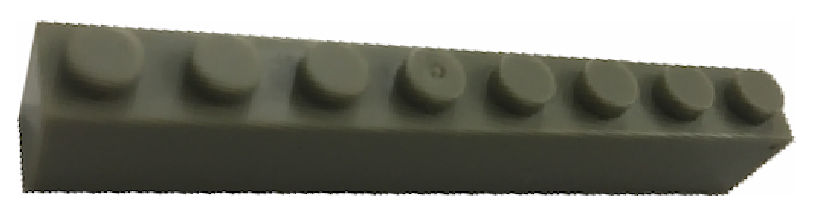
\includegraphics[width=5.4cm]{lego_8_1a} \qquad
            $j$ : 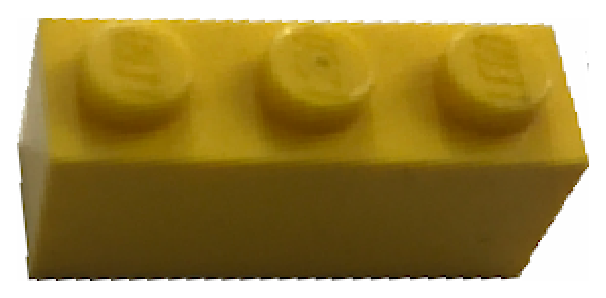
\includegraphics[width=1.98cm]{lego_3_1a} \qquad
            $k$ : 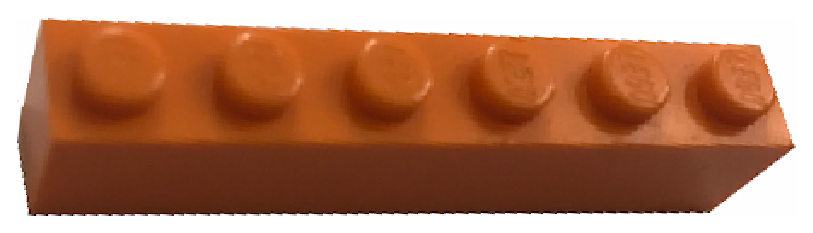
\includegraphics[width=4.05cm]{lego_6_1a} \\
            
      \partie[les fractions]
         \begin{enumerate}
            \item Compléter les égalités suivantes à l'aide de nombres entiers, décimaux ou fractionnaires : \\ [-3mm]
               \begin{multicols}{6}
                  $a = \pfh u$ \\ [7mm]
                  $b = \pfh u$ \\ [7mm]
                  $c = \pfh u$ \\ [7mm]
                  $d = \pfh u$ \\ [7mm]
                  $e = \pfh u$ \\ [7mm]
                  $f = \pfh u$ \\ [7mm]
                  $g = \pfh u$ \\ [7mm]
                  $h = \pfh u$ \\ [7mm]
                  $i = \pfh u$ \\ [7mm]
                  $j = \pfh u$ \\ [7mm]
                  $k = \pfh u$ \\ [7mm]
               \end{multicols} \medskip
            \item Compléter les égalités suivantes à l'aide de fractions dont le dénominateur est 8 : \\ [-3mm]
               \begin{multicols}{6}
                  $a = \dfrac{\qquad}{8} u$ \\ [7mm]
                  $b = \dfrac{\qquad}{8} u$ \\ [7mm]
                  $c = \dfrac{\qquad}{8} u$ \\ [7mm]
                  $d = \dfrac{\qquad}{8} u$ \\ [7mm]
                  $e = \dfrac{\qquad}{8} u$ \\ [7mm]
                  $f = \dfrac{\qquad}{8} u$ \\ [7mm]
                  $g = \dfrac{\qquad}{8} u$ \\ [7mm]
                  $h = \dfrac{\qquad}{8} u$ \\ [7mm]
                  $i = \dfrac{\qquad}{8} u$ \\ [7mm]
                  $j = \dfrac{\qquad}{8} u$ \\ [7mm]
                  $k = \dfrac{\qquad}{8} u$ \\ [7mm]
               \end{multicols} \smallskip
            \item Classer les Lego® dans l'ordre croissant de leur volume : \\ [2mm]
               \pf
      \end{enumerate}
   \end{QCM}
\end{activite}


%%%%%%%%%%%%%%%%%%%%%%%%%%%%%%%%%%%%%%%%%
%%%%%%%%%%%%%%%%%%%%%%%%%%%%%%%%%%%%%%%%%
\cours 

\section{Rappels sur les fractions} %%%

\begin{definition}
   Soit $a$ et $b$ deux nombres ($b\neq0$). Le {\bf quotient} $\dfrac{a}{b}$ est le nombre qui, multiplié par $b$, donne $a$. \\
   Ce quotient, écrit sous forme d'une fraction, est le résultat d'une division : $\dfrac{a}{b} =a\div b$.
\end{definition}

\begin{exemple}
   La fraction $\dfrac73$ peut-être interprétée comme :
   \correction
   \ \\ [-10mm]
   \begin{itemize}
      \item $7\div3$, dont une valeur approchée est 2,33 ;
      \item sept tiers, c'est-à-dire sept fois un tiers ;
      \item le nombre qui, multiplié par 3, donne
      7 : $\dfrac73\times3 =7$.
   \end{itemize}
\end{exemple}


\section{Égalité de fractions} %%%

\begin{propriete}
   On ne change pas la valeur d'une fraction en multipliant ou en divisant le numérateur et le dénominateur par un même nombre relatif non nul. \\ [1mm]
   \hspace*{3cm} $\dfrac{b}{c} =\dfrac{b\times a}{c\times a}= \dfrac{ba}{ca}. \text{\quad On a aussi \quad }a\times\dfrac{b}{c}= \dfrac{a\times b}{c} =\dfrac{ab}{c}$
\end{propriete}

%\begin{preuve}
%   {\hautab{1.9}
%   \begin{tabular}{p{3.7cm}p{10cm}}
%      $(a\times c)\times\dfrac{b}{c} =a\times \left(c\times\dfrac{b}{c}\right)$ & associativité de la multiplication\\
%      $\hspace*{16mm} =a\times b$
%      & $\dfrac{b}{c}$ est le nombre qui, multiplié par $c$ donne $b$ donc $c\times\dfrac{b}{c} =b$ \\
%      donc, $\dfrac{b}{c} =\dfrac{a\times b}{a\times c}$ & puisque $\dfrac{a\times b}{a\times c}$ est le nombre qui, multiplié par $a\times c$ donne $a\times b$ \\
%   \end{tabular}}
%\end{preuve}

\begin{exemple*1}   
   $\dfrac12 =\dfrac{1\times2}{2\times2} =\dfrac24 =\dfrac{2\times2}{4\times2} = \dfrac48\dots \qquad ; \qquad 7\times\dfrac{3}{5} =\dfrac{7\times3}{5} =\dfrac{21}{5}$.
\end{exemple*1}

\begin{remarque}
   la propriété permet de {\bf simplifier} des fractions, ce qui  signifie écrire une fraction qui lui est égale, mais avec un numérateur et un dénominateur plus petits.
\end{remarque}

\begin{exemple*1}
   Pour simplifier $\dfrac{150}{180}$, on peut tout d'abord diviser le numérateur et le dénominateur \\ [1mm]
      par 10 : $\dfrac{150}{180} =\dfrac{150\div10}{180\div10} =\dfrac{15}{18}$, puis les diviser encore par 3 : $\dfrac{15}{18} =\dfrac{15\div3}{18\div3} =\dfrac56$.
\end{exemple*1}


\section{Comparaison de fractions} %%%

\begin{propriete}
   \begin{itemize}
      \item Pour comparer deux fractions ayant le même dénominateur, on compare uniquement le numérateur : la fraction la plus grande est celle dont le numérateur est le plus grand.
      \item Pour comparer deux fractions de dénominateurs différents, on modifie l'écriture des fractions pour qu'elles aient le même dénominateur. \\ [-8mm]
   \end{itemize}
\end{propriete}

\begin{exemple}
   Comparer les fractions suivantes : \smallskip
   \begin{itemize}
      \item $\dfrac35$ et $\dfrac45$. \medskip
      \item $\dfrac23$ et $\dfrac{7}{12}$.
   \end{itemize}
   \correction
   On a :
   \begin{itemize}
      \item $3<4$ donc $\dfrac35<\dfrac45$. \smallskip
      \item On remarque que $\dfrac23=\dfrac{2\times4}{3\times4}=\dfrac{8}{12}$. \\ [1mm]
      Comme $\dfrac{8}{12}>\dfrac{7}{12}$, alors $\dfrac23>\dfrac{7}{12}$.
   \end{itemize}
\end{exemple}


%%%%%%%%%%%%%%%%%%%%%%%%%%%%%%%%%%%%%%%%%%
%%%%%%%%%%%%%%%%%%%%%%%%%%%%%%%%%%%%%%%%%%
\exercicesbase

\begin{colonne*exercice}

\serie{Fractions}

\begin{exercice} %1
   Ecrire la fraction qui représente la partie colorée de chaque figure puis la simplifier si possible. \\
   \begin{center}
      {\psset{unit=0.6}
      \begin{pspicture}(-1,-1.5)(2.2,1)
         \psframe[fillstyle=solid,fillcolor=A2](0,0)(-1,-1)
         \psframe(-1,-1)(1,1)
         \psline(-1,0)(1,0)
         \psline(0,-1)(0,1)
         \rput(-1.4,0){$a$}
      \end{pspicture}
      \begin{pspicture}(-1,-1.5)(2.2,1)
         \pspolygon[fillstyle=solid,fillcolor=A2](0,0)(0,-1)(1,-1)(1,1)(1,1)(-1,1)(-1,0)
         \psframe(-1,-1)(1,1)
         \psline(-1,0)(1,0)
         \psline(0,-1)(0,1)
         \rput(-1.4,0){$b$}
      \end{pspicture}
      \begin{pspicture}(-1,-1.5)(2.2,1)
         \psframe[fillstyle=solid,fillcolor=A2](-1,-1)(1,0)
         \psframe(-1,-1)(1,1)
         \psline(-1,0)(1,0)
         \psline(0,-1)(0,1)
         \rput(-1.4,0){$c$}
      \end{pspicture}
      \begin{pspicture}(-1,-1.5)(1,1)
         \psframe[fillstyle=solid,fillcolor=A2](-1,-1)(1,1)
         \psline(-1,0)(1,0)
         \psline(0,-1)(0,1)
         \rput(-1.4,0){$d$}
      \end{pspicture} \\ \medskip
      
      \begin{pspicture}(-1,-1.5)(2.2,1)
         \pswedge[fillstyle=solid,fillcolor=B2](0,0){1}{30}{-30}
         \pscircle(0,0){1}
         \multido{\n=0+30}{12}{\psline(0,0)(1;\n)}
         \rput(-1.4,0){$e$}
      \end{pspicture}
      \begin{pspicture}(-1,-1.5)(2.2,1)
         \pswedge[fillstyle=solid,fillcolor=B2](0,0){1}{90}{180}
         \pscircle(0,0){1}
         \multido{\n=0+30}{12}{\psline(0,0)(1;\n)}
         \rput(-1.4,0){$f$}
      \end{pspicture}
      \begin{pspicture}(-1,-1.5)(2.2,1)
         \pswedge[fillstyle=solid,fillcolor=B2](0,0){1}{-120}{-60}
         \pscircle(0,0){1}
         \multido{\n=0+30}{12}{\psline(0,0)(1;\n)}
         \rput(-1.4,0){$g$}
      \end{pspicture}
      \begin{pspicture}(-1,-1.5)(1,1)
         \pswedge[fillstyle=solid,fillcolor=B2](0,0){1}{60}{-120}
         \pscircle(0,0){1}
         \multido{\n=0+30}{12}{\psline(0,0)(1;\n)}
         \rput(-1.4,0){$h$}
      \end{pspicture} \\ \medskip
      
      \begin{pspicture}(-1,-1.2)(2.2,1.3)
         \pspolygon[fillstyle=solid,fillcolor=H1](1.2;210)(0,-0.6)(1.2;90)
         \pspolygon(1.2;-30)(1.2;90)(1.2;210)
         \psline(0.6;150)(1.2;-30)
         \psline(0.6;30)(1.2;210)
         \psline(0,-0.6)(0,1.2)
         \rput(-1.4,0.25){$i$}
      \end{pspicture}
      \begin{pspicture}(-1,-1.2)(2.2,1.3)
         \pspolygon[fillstyle=solid,fillcolor=H1](0,0)(1.2;-30)(0,-0.6)
         \pspolygon[fillstyle=solid,fillcolor=H1](0,0)(1.2;210)(0.6;150)
         \pspolygon[fillstyle=solid,fillcolor=H1](0,0)(1.2;90)(0.6;30)
         \pspolygon(1.2;-30)(1.2;90)(1.2;210)
         \psline(0.6;150)(1.2;-30)
         \psline(0.6;30)(1.2;210)
         \psline(0,-0.6)(0,1.2)
         \rput(-1.4,0.25){$j$}
      \end{pspicture}
      \begin{pspicture}(-1,-1.2)(2.2,1.3)
         \pspolygon[fillstyle=solid,fillcolor=H1](0,0)(0.6;30)(1.2;90)(0.6;150)
         \pspolygon(1.2;-30)(1.2;90)(1.2;210)
         \psline(0.6;150)(1.2;-30)
         \psline(0.6;30)(1.2;210)
         \psline(0,-0.6)(0,1.2)
         \rput(-1.4,0.25){$k$}
      \end{pspicture}
      \begin{pspicture}(-1,-1.2)(1,1.3)
         \pspolygon[fillstyle=solid,fillcolor=H1](0,0)(0.6;30)(1.2;90)(1.2;210)(1.2;-30)
         \pspolygon(1.2;-30)(1.2;90)(1.2;210)
         \psline(0.6;150)(1.2;-30)
         \psline(0.6;30)(1.2;210)
         \psline(0,-0.6)(0,1.2)
         \rput(-1.4,0.25){$l$}
      \end{pspicture} \\ \medskip
      
      \begin{pspicture}(-1,-1.5)(2.2,1)
         \psgrid[subgriddiv=2,subgridcolor=black,subgridwidth=0.8pt,gridlabels=0](-1,-1)(1,1)
         \psframe[fillstyle=solid,fillcolor=J1](-1,0)(0,1)
         \rput(-1.4,0){$m$}
      \end{pspicture}
      \begin{pspicture}(-1,-1.5)(2.2,1)
         \psgrid[subgriddiv=2,subgridcolor=black,subgridwidth=0.8pt,gridlabels=0](-1,-1)(1,1)
         \psframe[fillstyle=solid,fillcolor=J1](-1,0)(0,1)
         \psframe[fillstyle=solid,fillcolor=J1](0,0.5)(0.5,0)
         \psframe[fillstyle=solid,fillcolor=J1](-1,-0.5)(-0.5,0)
         \rput(-1.4,0){$n$}
      \end{pspicture}
      \begin{pspicture}(-1,-1.5)(2.2,1)
         \psgrid[subgriddiv=2,subgridcolor=black,subgridwidth=0.8pt,gridlabels=0](-1,-1)(1,1)
         \psframe[fillstyle=solid,fillcolor=J1](-1,-1)(1,0)
         \psframe[fillstyle=solid,fillcolor=J1](-1,0)(0,1)
         \psframe[fillstyle=solid,fillcolor=J1](0,0)(0.5,0.5)
         \rput(-1.4,0){$p$}
      \end{pspicture}
      \begin{pspicture}(-1,-1.5)(1,1)
         \psgrid[subgriddiv=2,subgridcolor=black,subgridwidth=0.8pt,gridlabels=0](-1,-1)(1,1)
         \psframe[fillstyle=solid,fillcolor=J1](-1,-1)(0.5,0)
         \psframe[fillstyle=solid,fillcolor=J1](-1,0)(-0.5,1)
         \psframe[fillstyle=solid,fillcolor=J1](0.5,-0.5)(1,0)
         \rput(-1.4,0){$q$}
      \end{pspicture}}   
   \end{center}
\end{exercice}
      
\begin{corrige}
   \begin{colitemize}{3}
      \item $a =\blue \dfrac14$ \medskip
      \item $b =\blue \dfrac34$ \medskip
      \item $c =\blue \dfrac24 =\dfrac12$ \medskip
      \item $d =\blue \dfrac44 =1$ \medskip
      \item $e =\blue \dfrac{10}{12} =\dfrac56$ \medskip
      \item $f =\blue \dfrac{3}{12} =\dfrac14$
      \item $g =\blue \dfrac{2}{12} =\dfrac16$
      \item $h =\blue \dfrac{6}{12} =\dfrac12$
      \item $i =\blue \dfrac36 =\dfrac12$
      \item $j =\blue \dfrac36 =\dfrac12$
      \item $k =\blue \dfrac26 =\dfrac13$
      \item $l =\blue \dfrac56$
      \item $m =\blue \dfrac{4}{16} =\dfrac14$
      \item $n =\blue \dfrac{6}{16} =\dfrac38$
      \item $p =\blue \dfrac{13}{16}$
      \item $q =\blue \dfrac{9}{16}$
   \end{colitemize}
\end{corrige}
    
      
\begin{exercice} %2
   Dans chaque figure ci-dessous, colorier selon la fraction donnée.
   \begin{center}
   {\small
      \psset{unit=0.75}
      \begin{pspicture}(-1,-1.3)(2.5,1)
         \psframe(-1,-1)(1,1)
         \rput(1.25,0){$\dfrac13$}
      \end{pspicture}
      \begin{pspicture}(-1,-1.3)(2.5,1)
         \psframe(-1,-1)(1,1)
         \rput(1.25,0){$\dfrac34$}
      \end{pspicture}
      \begin{pspicture}(-1,-1.3)(1.5,1)
         \psframe(-1,-1)(1,1)
         \rput(1.25,0){$\dfrac58$}
      \end{pspicture} \\ \medskip
      
      \begin{pspicture}(-1,-1.3)(2.5,1)
         \pscircle(0,0){1}
         \rput(1.25,0){$\dfrac13$}
      \end{pspicture}
      \begin{pspicture}(-1,-1.3)(2.5,1)
         \pscircle(0,0){1}
         \rput(1.25,0){$\dfrac34$}
      \end{pspicture}
      \begin{pspicture}(-1,-1.3)(1.5,1)
         \pscircle(0,0){1}
         \rput(1.25,0){$\dfrac58$}
      \end{pspicture} \\ \medskip
      
      \begin{pspicture}(-1,-1.3)(2.5,1)
         \pspolygon(1;30)(1;90)(1;150)(1;210)(1;270)(1;330)
         \rput(1.25,0){$\dfrac13$}
      \end{pspicture}
      \begin{pspicture}(-1,-1.3)(2.5,1)
         \pspolygon(1;30)(1;90)(1;150)(1;210)(1;270)(1;330)
         \rput(1.25,0){$\dfrac34$}
      \end{pspicture}
      \begin{pspicture}(-1,-1.3)(1.5,1)
         \pspolygon(1;30)(1;90)(1;150)(1;210)(1;270)(1;330)
         \rput(1.25,0){$\dfrac56$}
      \end{pspicture} \\ \medskip

      \begin{pspicture}(-1,-1.3)(2.5,1)
         \pspolygon(-1,-0.33)(-1,0.33)(-0.33,0.33)(-0.33,1)(0.33,1)(0.33,0.33)(1,0.33)(1,-0.33)(0.33,-0.33)(0.33,-1)(-0.33,-1)(-0.33,-0.33)
         \rput(1.25,0){$\dfrac14$}
      \end{pspicture}
      \begin{pspicture}(-1,-1.3)(2.5,1)
         \pspolygon(-1,-0.33)(-1,0.33)(-0.33,0.33)(-0.33,1)(0.33,1)(0.33,0.33)(1,0.33)(1,-0.33)(0.33,-0.33)(0.33,-1)(-0.33,-1)(-0.33,-0.33)
         \rput(1.25,0){$\dfrac38$}
      \end{pspicture}
      \begin{pspicture}(-1,-1.3)(1.5,1)
         \pspolygon(-1,-0.33)(-1,0.33)(-0.33,0.33)(-0.33,1)(0.33,1)(0.33,0.33)(1,0.33)(1,-0.33)(0.33,-0.33)(0.33,-1)(-0.33,-1)(-0.33,-0.33)
         \rput(1.25,0){$\dfrac25$}
      \end{pspicture}}
   \end{center}
\end{exercice}

\begin{corrige}
   \ \\ [-3mm]
   {\small
      \psset{unit=0.6}
      \begin{pspicture}(-1,-1.2)(3,1)
         \psframe(-1,-1)(1,1)
         \psline(-0.33,-1)(-0.33,1)
         \psline(0.33,-1)(0.33,1)
         \psframe[fillstyle=solid,fillcolor=A2](-1,-1)(-0.33,1)
         \rput(1.5,0){$\dfrac13$}
      \end{pspicture}
      \begin{pspicture}(-1,-1.2)(3,1)
         \pspolygon[fillstyle=solid,fillcolor=A2](0,0)(0,-1)(1,-1)(1,1)(1,1)(-1,1)(-1,0)
         \psframe(-1,-1)(1,1)
         \psline(-1,0)(1,0)
         \psline(0,-1)(0,1)
         \rput(1.5,0){$\dfrac34$}
      \end{pspicture}
      \begin{pspicture}(-1,-1.2)(1.5,1)
         \pspolygon[fillstyle=solid,fillcolor=A2](0,0)(1,-1)(1,-1)(1,1)(1,1)(-1,1)(-1,0)
         \psframe(-1,-1)(1,1)
         \psline(-1,0)(1,0)
         \psline(0,-1)(0,1)
         \psline(-1,-1)(1,1)
         \psline(-1,1)(1,-1)
         \rput(1.5,0){$\dfrac58$}
      \end{pspicture} \\ \medskip
      
      \begin{pspicture}(-1,-1.2)(3,1)
         \pswedge[fillstyle=solid,fillcolor=B2](0,0){1}{0}{120}
         \pscircle(0,0){1}
         \multido{\n=0+120}{3}{\psline(0,0)(1;\n)}
         \rput(1.5,0){$\dfrac13$}
      \end{pspicture}
      \begin{pspicture}(-1,-1.2)(3,1)
         \pswedge[fillstyle=solid,fillcolor=B2](0,0){1}{0}{-90}
         \pscircle(0,0){1}
         \multido{\n=0+90}{4}{\psline(0,0)(1;\n)}
         \rput(1.5,0){$\dfrac34$}
      \end{pspicture}
      \begin{pspicture}(-1,-1.2)(1.5,1)
         \pswedge[fillstyle=solid,fillcolor=B2](0,0){1}{0}{225}
         \pscircle(0,0){1}
         \multido{\n=0+45}{8}{\psline(0,0)(1;\n)}
         \rput(1.5,0){$\dfrac58$}
      \end{pspicture} \\ \medskip
      
      \begin{pspicture}(-1,-1.2)(3,1)
         \pspolygon[fillstyle=solid,fillcolor=H1](0,0)(1;30)(1;90)(1;150)
         \multido{\n=30+120}{3}{\psline(0,0)(1;\n)}
         \pspolygon(1;30)(1;90)(1;150)(1;210)(1;270)(1;330)
         \rput(1.5,0){$\dfrac13$}
      \end{pspicture}
      \begin{pspicture}(-1,-1.2)(3,1)
         \pspolygon[fillstyle=solid,fillcolor=H1](1;30)(1;90)(1;150)(1;210)(1;270)(1;330)
         \pspolygon[fillstyle=solid,fillcolor=white](0,0)(0.87,0)(1;30)(0,1)
         \psline(0,-1)(0,1)
         \psline(-0.87,0)(0.87,0)
         \rput(1.5,0){$\dfrac34$}
      \end{pspicture}
      \begin{pspicture}(-1,-1.2)(1.5,1)
         \pspolygon[fillstyle=solid,fillcolor=H1](1;30)(1;90)(1;150)(1;210)(1;270)(1;330)
         \pspolygon[fillstyle=solid,fillcolor=white](0,0)(1;30)(0,1)
         \multido{\n=30+60}{6}{\psline(0,0)(1;\n)}
         \rput(1.5,0){$\dfrac56$}
      \end{pspicture} \\ \medskip

      \begin{pspicture}(-1,-1.5)(3,1)
         \pspolygon[fillstyle=solid,fillcolor=J1](0,0)(0.33,0.33)(0.33,1)(-0.33,1)(-0.33,0.33)
         \pspolygon(-1,-0.33)(-1,0.33)(-0.33,0.33)(-0.33,1)(0.33,1)(0.33,0.33)(1,0.33)(1,-0.33)(0.33,-0.33)(0.33,-1)(-0.33,-1)(-0.33,-0.33)
         \psline(-0.33,-0.33)(0.33,0.33)
         \psline(0.33,-0.33)(-0.33,0.33)
         \rput(1.5,0){$\dfrac14$}
      \end{pspicture}
      \begin{pspicture}(-1,-1.5)(3,1)
         \pspolygon[fillstyle=solid,fillcolor=J1](0,0)(1,0)(1,0.33)(0.33,0.33)(0.33,1)(-0.33,1)(-0.33,0.33)
         \pspolygon(-1,-0.33)(-1,0.33)(-0.33,0.33)(-0.33,1)(0.33,1)(0.33,0.33)(1,0.33)(1,-0.33)(0.33,-0.33)(0.33,-1)(-0.33,-1)(-0.33,-0.33)
         \pspolygon(-1,-0.33)(-1,0.33)(-0.33,0.33)(-0.33,1)(0.33,1)(0.33,0.33)(1,0.33)(1,-0.33)(0.33,-0.33)(0.33,-1)(-0.33,-1)(-0.33,-0.33)
         \psline(-0.33,-0.33)(0.33,0.33)
         \psline(0.33,-0.33)(-0.33,0.33)
         \psline(-1,0)(1,0)
         \psline(0,-1)(0,1)
         \rput(1.5,0){$\dfrac38$}
      \end{pspicture}
      \begin{pspicture}(-1,-1.5)(1.5,1)
         \psframe[fillstyle=solid,fillcolor=J1](-0.33,-0.33)(1,0.33)
         \pspolygon(-1,-0.33)(-1,0.33)(-0.33,0.33)(-0.33,1)(0.33,1)(0.33,0.33)(1,0.33)(1,-0.33)(0.33,-0.33)(0.33,-1)(-0.33,-1)(-0.33,-0.33)
         \psframe(-0.33,-0.33)(0.33,0.33)
         \rput(1.5,0){$\dfrac25$}
      \end{pspicture}}
\end{corrige}

%%%%%%%%%%%%%
\serie{Egalités et comparaisons}

\begin{exercice} %3
   Compléter avec le signe $=$ ou $\neq$. \medskip
   \begin{colenumerate}{3}
      \item $\dfrac{3+5}{7+5} \pfh \dfrac{3}{7}$ \bigskip
      \item $\dfrac{3\times5}{7\times5} \pfh \dfrac{3}{7}$ \bigskip
      \item $\dfrac{3\times7}{7\times3} \pfh \dfrac{3}{7}$ \medskip
      \item $\dfrac{33}{77} \pfh \dfrac{3}{7}$
      \item $\dfrac{7}{3} \pfh \dfrac{3}{7}$
      \item $\dfrac{3}{7} \pfh 3,7$
      \item $\dfrac{3}{7} \pfh \dfrac{30}{70}$
      \item $\dfrac{3}{3} \pfh \dfrac{7}{7}$
      \item $3 \pfh\dfrac{21}{7}$
   \end{colenumerate}
\end{exercice}

\begin{corrige}
    \begin{colenumerate}{3}
      \item $\dfrac{3+5}{7+5} \, {\blue \neq} \, \dfrac{3}{7}$ \medskip
      \item $\dfrac{3\times5}{7\times5} \, {\blue =} \, \dfrac{3}{7}$ \medskip
      \item $\dfrac{3\times7}{7\times3} \, {\blue \neq} \, \dfrac{3}{7}$ \medskip
      \item $\dfrac{33}{77} \, {\blue =} \,  \dfrac{3}{7}$
      \item $\dfrac{7}{3} \, {\blue \neq} \, \dfrac{3}{7}$
      \item $\dfrac{3}{7} \, {\blue \neq} \, 3,7$
      \item $\dfrac{3}{7} \, {\blue =} \, \dfrac{30}{70}$
      \item $\dfrac{3}{3} \, {\blue =} \, \dfrac{7}{7}$
      \item $3 \, {\blue =} \, \dfrac{21}{7}$
   \end{colenumerate}
\end{corrige}

\medskip

%\begin{exercice} %3
%   Par quel nombre faut-il :
%   \begin{enumerate}
%      \item multiplier 5 pour obtenir 3 ?
%      \item multiplier 19 pour obtenir 97 ?
%      \item multiplier 12 pour obtenir 11 ?
%   \end{enumerate}
%   Ecrire à chaque fois l'égalité obtenue.
%\end{exercice}
%
%\begin{corrige}
%   \ \\ [-5mm]
%   \begin{enumerate}
%      \item On multiplie 5 par $\blue\dfrac35$ pour obtenir 3 : $5\times\dfrac35 =3$. \smallskip
%      \item On multiplie 19 par $\blue\dfrac{97}{19}$ pour obtenir 97 : \\
%          \qquad $19\times\dfrac{97}{19} =97$.
%      \item On multiplie 12 par $\blue\dfrac{11}{12}$ pour obtenir 11 : \\
%         \qquad $12\times\dfrac{11}{12} =11$.
%   \end{enumerate}
%\end{corrige}


\begin{exercice} %4
   Compléter les fractions suivantes : \medskip
   \begin{enumerate}
      \item $\dfrac{1}{2} =\dfrac{\qquad\;}{14} =\dfrac{8}{\qquad\;} =\dfrac{\qquad\;}{50} =\dfrac{16}{\qquad\;} =\dfrac{64}{\qquad\;}$ \\ [2mm]
      \item $\dfrac{4}{5} =\dfrac{\qquad\;}{15} =\dfrac{8}{\qquad\;} =\dfrac{\qquad\;}{50} =\dfrac{16}{\qquad\;} =\dfrac{64}{\qquad\;}$ \\ [2mm]
      \item $\dfrac{11}{7} =\dfrac{\qquad\;}{14} =\dfrac{88}{\qquad\;} =\dfrac{\qquad\;}{49} =\dfrac{121}{\qquad\;} =\dfrac{550}{\qquad\;}$ \\
   \end{enumerate}
\end{exercice}

\begin{corrige}
   \ \\ [-5mm]
   \begin{enumerate}
      \item $\dfrac{1}{2} =\dfrac{\blue 7}{14} =\dfrac{8}{\blue 16} =\dfrac{\blue 25}{50} =\dfrac{16}{\blue 32} =\dfrac{64}{\blue 128}$ \\ [2mm]
      \item $\dfrac{4}{5} =\dfrac{\blue 12}{15} =\dfrac{8}{\blue 10} =\dfrac{\blue 40}{50} =\dfrac{16}{\blue 20} =\dfrac{64}{\blue 80}$ \\ [2mm]
      \item $\dfrac{11}{7} =\dfrac{\blue 22}{14} =\dfrac{88}{\blue 56} =\dfrac{\blue 77}{49} =\dfrac{121}{\blue 77} =\dfrac{550}{\blue 350}$
   \end{enumerate}
\end{corrige}

\medskip

\begin{exercice} %5
   Surligner d'une même couleur les nombres égaux. \\ [2mm]
   {\hautab{2}
   \begin{tabular}{|*{7}{C{0.8}}|}
      \hline
      $\dfrac{5}{4}$ & $\dfrac{54}{45}$ & $\dfrac{28}{42}$ & $\dfrac{12}{15}$ & $\dfrac{1}{2}$ & $\dfrac{9}{81}$ & $\dfrac{4}{6}$ \\ [2mm]
      $\dfrac{50}{40}$ & $\dfrac{27}{54}$ & $\dfrac{4}{36}$ & $\dfrac{36}{72}$ & $\dfrac{1}{9}$ & $\dfrac{4}{5}$ & $\dfrac{6}{5}$ \\ [2mm]
      \hline
   \end{tabular}} \\ [1mm]
\end{exercice}

\begin{corrige}
   \ \\ [-8mm]
   {\hautab{2}
   \begin{tabular}[t]{|*{7}{C{0.6}}|}
      \hline
      $\textcolor{red}{\dfrac{5}{4}}$ & $\textcolor{blue}{\dfrac{54}{45}}$ & $\textcolor{orange}{\dfrac{28}{42}}$ & $\textcolor{green}{\dfrac{12}{15}}$ & $\textcolor{violet}{\dfrac{1}{2}}$ & $\textcolor{teal}{\dfrac{9}{81}}$ & $\textcolor{orange}{\dfrac{4}{6}}$ \\
       $\textcolor{red}{\dfrac{50}{40}}$ & $\textcolor{violet}{\dfrac{27}{54}}$ & $\textcolor{teal}{\dfrac{4}{36}}$ & $\textcolor{violet}{\dfrac{36}{72}}$ & $\textcolor{teal}{\dfrac{1}{9}}$ & $\textcolor{green}{\dfrac{4}{5}}$ & $\textcolor{blue}{\dfrac{6}{5}}$ \\ [1mm]
      \hline
   \end{tabular}}
\end{corrige}

\medskip

\begin{exercice} %6
   Simplifier au maximum ces fractions. \medskip
   \begin{colenumerate}{4}
      \item $\dfrac{6}{10}$ \bigskip
      \item $\dfrac{18}{16}$ \bigskip
      \item $\dfrac{16}{28}$
      \item $\dfrac{30}{48}$
      \item $\dfrac{88}{33}$
      \item $\dfrac{55}{30}$
      \item $\dfrac{15}{75}$
      \item $\dfrac{108}{117}$
   \end{colenumerate}
\end{exercice}

\begin{corrige}
   \begin{colenumerate}{2}
      \item $\dfrac{6}{10} =\dfrac{\cancel2\times3}{\cancel2\times5} =\blue\dfrac35$ \medskip
      \item $\dfrac{18}{16} =\dfrac{\cancel2\times9}{\cancel2\times8} =\blue\dfrac98$ \medskip
      \item $\dfrac{16}{28} =\dfrac{\cancel4\times4}{\cancel4\times7} =\blue\dfrac47$ \medskip
      \item $\dfrac{30}{48} =\dfrac{\cancel6\times5}{\cancel6\times8} =\blue\dfrac58$ \medskip
      \item $\dfrac{88}{33} =\dfrac{\cancel{11}\times8}{\cancel{11}\times3} =\blue\dfrac83$ \medskip
      \item $\dfrac{55}{30} =\dfrac{\cancel5\times11}{\cancel5\times6} =\blue\dfrac{11}6$ \medskip
      \item $\dfrac{15}{75} =\dfrac{\cancel{15}\times1}{\cancel{15}\times5} =\blue\dfrac15$ \medskip
      \item $\dfrac{108}{117} =\dfrac{\cancel9\times12}{\cancel9\times13} =\blue\dfrac{12}{13}$
   \end{colenumerate}
\end{corrige}

\medskip

\begin{exercice} %7
   Comparer les fractions suivantes : \medskip
   \begin{colenumerate}{3}
      \item $\dfrac{1}{9} \pfh \dfrac{1}{3}$ \bigskip
      \item $\dfrac{4}{9} \pfh \dfrac{12}{9}$ \bigskip
      \item $\dfrac{18}{17} \pfh 1$ \bigskip
      \item $\dfrac{7}{19} \pfh \dfrac{7}{20}$
      \item $\dfrac{2}{3} \pfh \dfrac{4}{6}$
      \item $\dfrac{18}{13} \pfh \dfrac{15}{13}$
      \item $\dfrac{81}{91} \pfh \dfrac{81}{90}$
      \item $\dfrac{17}{10} \pfh 0,7$
      \item $\dfrac{2}{3} \pfh \dfrac{1}{4}$
   \end{colenumerate}
\end{exercice}

\begin{corrige}
   \begin{colenumerate}{3}
      \item $\dfrac{1}{9} \, {\blue <} \, \dfrac{1}{3}$ \smallskip
      \item $\dfrac{4}{9} \, {\blue <} \,\dfrac{12}{9}$ \smallskip
      \item $\dfrac{18}{17} \, {\blue >} \,1$
      \item $\dfrac{7}{19} \, {\blue >} \,\dfrac{7}{20}$
      \item $\dfrac{2}{3} \, {\blue =} \,\dfrac{4}{6}$
      \item $\dfrac{18}{13} \, {\blue >} \,\dfrac{15}{13}$
      \item $\dfrac{81}{91} \, {\blue <} \,\dfrac{81}{90}$
      \item $\dfrac{17}{10} \, {\blue >} \,0,7$
      \item $\dfrac{2}{3} \, {\blue >} \,\dfrac{1}{4}$
   \end{colenumerate}
\end{corrige}

\medskip

\begin{exercice} %8
   Pour chaque item, réduire les fractions au même dénominateur, les ranger dans l'ordre croissant puis en déduire le classement des fractions initiales dans l'ordre croissant. \medskip
   \begin{enumerate}
      \item $A =\dfrac12 \; ; \; B =\dfrac23 \; ; \; C =\dfrac56 \; ; \; D = \dfrac5{12} \; ; \; E =\dfrac7{24}$. \bigskip
      \item $F =\dfrac12 \; ; \; G =\dfrac34 \; ; \; H =\dfrac78 \; ; \; I = \dfrac{11}{16} \; ; \; J =\dfrac{23}{32}$.
   \end{enumerate}
\end{exercice}

\begin{corrige}
   \ \\ [-5mm]
   \begin{enumerate}
      \item Fractions de dénominateur 24. \\ [1.5mm]
         $A =\dfrac{1\times12}{2\times12} =\dfrac{12}{24} \qquad B =\dfrac{2\times8}{3\times8} =\dfrac{16}{24}$ \\ [1.5mm]
         $C =\dfrac{5\times4}{6\times4} =\dfrac{20}{24} \qquad D = \dfrac{5\times2}{12\times2} =\dfrac{10}{24} \qquad E =\dfrac{7}{24}$ \\ [1.5mm]
         $\dfrac{7}{24}<\dfrac{10}{24}<\dfrac{12}{24}<\dfrac{16}{24}<\dfrac{20}{24}\Rightarrow$ {\blue $E<D<A<B<C$} \\ [3mm]
      \item Fractions de dénominateur 32. \\ [1.5mm]
         $F =\dfrac{1\times16}{2\times16} =\dfrac{16}{32} \qquad G =\dfrac{3\times8}{4\times8} =\dfrac{24}{32}$ \\ [1.5mm]
         $H =\dfrac{7\times4}{8\times4} =\dfrac{28}{32} \qquad I = \dfrac{11\times2}{16\times2} =\dfrac{22}{32} \qquad J =\dfrac{23}{32}$ \\ [1.5mm]
         $\dfrac{16}{32}<\dfrac{22}{32}<\dfrac{23}{32}<\dfrac{23}{32}<\dfrac{24}{32} \Rightarrow$ {\blue $F<I<J<G<H$} \\ [3mm]
   \end{enumerate}
   
\bigskip
\corec{ExploRATIO}
\bigskip

   \begin{ltableau}{\linewidth}{8}
      \hline
      \multicolumn{8}{|c|}{Niveau 1} \\
      \hline
      1a & 1b & 1c & 1d & 1e & 1f & 1g & 1h \\
      \hline
      & & & & & & & \\ [-4mm]
      $\dfrac27$ & $\dfrac38$ & $\dfrac14 $ & $\dfrac25$ & $\dfrac78$ & $\dfrac34$ & $\dfrac76$ & $\dfrac75$ \\
      & & & & & & & \\ [-4mm]
      \hline
   \end{ltableau}
   
   \begin{ltableau}{\linewidth}{8}
      \hline
      \multicolumn{8}{|c|}{Niveau 2} \\
      \hline
      2a & 2b & 2c & 2d & 2e & 2f & 2g & 2h \\
      \hline
      & & & & & & & \\ [-4mm]
      $\dfrac14$ & $\dfrac18$ & $\dfrac16$ & $\dfrac{1}{18}$ & $\dfrac{11}{24}$ & $\dfrac13$ & $\dfrac89$ & $\dfrac13$ \\
      & & & & & & & \\ [-4mm]
      \hline
   \end{ltableau}
   
   \begin{ltableau}{\linewidth}{7}
      \hline
      \multicolumn{7}{|c|}{Niveau 3} \\
      \hline
      2i & 2j & 2k & 2l & 2m & 2n & 2p \\
      \hline
      & & & & & & \\ [-4mm]
      $\dfrac{13}{6}$ & $\dfrac23$ & $\dfrac35$ & $\dfrac23$ & $1$ & $\dfrac12$ & $\dfrac38$ \\
      & & & & & & \\ [-4mm]
      \hline
   \end{ltableau}
\end{corrige}


\end{colonne*exercice}


%%%%%%%%%%%%%%%%%%%%%%%%%%%%%%%%%%%%%%%%%%
\Recreation

\enigme[ExploRATIO]
   \partie[présentation du matériel] 
      ExploRATIO est un matériel permettant des activités de manipulation et de réflexion dans le domaine des fractions. \\
      Il est composé de {\bf transparents} représentant un carré unité, puis un carré partagé en 2, en 3, en 4, en 5, en 6, en 7, en 8, en 9 et en 10 et de {\bf vignettes} dont une partie est colorée. \\
      L'objectif est de déterminer la fraction de l'unité correspondant à la partie colorée. \\ [3mm]
      {\it Exemple de vignette :
      \begin{center}
         \psset{unit=0.5}
         \begin{pspicture}(0,-1)(30,10)
            \psframe(0,0)(10,10)
            \psset{fillstyle=solid,fillcolor=A1}
            \psframe[linecolor=A1](1.43,0)(5.71,10)
            \rput(15,5){\parbox{4cm}{le transparent divisé en 7 parts égales permet de vérifier que la partie colorée correspond à trois septièmes d'unité, soit $\dfrac37$.}}
            \psframe[fillcolor=lightgray!50](20,0)(30,10)
            \psframe(21.43,0)(25.71,10)
            \multido{\n=21.43+1.43}{6}{\psline(\n,0)(\n,10)}
            \rput(29.6,9.5){7}
            \rput{90}(20.6,1.8){\footnotesize\gray ExploRATIO}
         \end{pspicture}
       \end{center}}

   \partie[À vous de jouer !]
      Pour chacun des niveaux 1, 2 et 3, donner la fraction de carré unité coloriée puis simplifier au maximum.
      \begin{center}
         \begin{ltableau}{\linewidth}{8}
            \hline
            \multicolumn{8}{|c|}{Niveau 1} \\
            \hline
            1a & 1b & 1c & 1d & 1e & 1f & 1g & 1h \\
            \hline
            & & & & & & & \\
            & & & & & & & \\
            & & & & & & & \\
            \hline
         \end{ltableau}
         \bigskip
         \begin{ltableau}{\linewidth}{8}
            \hline
            \multicolumn{8}{|c|}{Niveau 2} \\
            \hline
            2a & 2b & 2c & 2d & 2e & 2f & 2g & 2h \\
            \hline
            & & & & & & & \\
            & & & & & & & \\
            & & & & & & & \\
            \hline
         \end{ltableau}
         \bigskip
         \begin{ltableau}{\linewidth}{7}
            \hline
            \multicolumn{7}{|c|}{Niveau 3} \\
            \hline
            2i & 2j & 2k & 2l & 2m & 2n & 2p \\
            \hline
            & & & & & & \\
            & & & & & & \\
            & & & & & & \\
            \hline
         \end{ltableau}
      \end{center}
      
  
\vfill\hfill{\footnotesize \href{https://wp.gem-math.be/2021/02/04/exploratio-2/}{ExploRATIO : Un dispositif pédagogique créé par le 
Groupe d’Enseignement Mathématique (Belgique)}}

